\documentclass[3p, a4paper, authoryear, 11pt, fleqn, review]{elsarticle}
\usepackage{acronym}
\usepackage[linesnumbered, ruled, vlined]{algorithm2e}
\usepackage{amsmath,amssymb,amsfonts}
\usepackage{siunitx}
\usepackage{graphicx}
\graphicspath{
	{./graphics/}
}
\usepackage{hyperref}

\usepackage[left,mathlines]{lineno}
\usepackage{enumitem}
\usepackage[normalem]{ulem}
\usepackage{pdflscape}


\usepackage{natbib}
	\bibliographystyle{apalike}

\hypersetup{
  	bookmarks=true,         % show bookmarks bar?
    unicode=false,          % non-Latin characters in Acrobat's bookmarks
    pdftoolbar=true,        % show Acrobat's toolbar?
    pdfmenubar=true,        % show Acrobat's menu?
    pdffitwindow=true,      % page fit to window when opened
    pdftitle={}, 	% title
    pdfauthor={},   % author
    pdfsubject={},% subject of the document
    pdfnewwindow=true,      % links in new window
    pdfkeywords={},			%list of keywords
    colorlinks=true,   		% false: boxed links; true: colored links
    linkcolor=blue,        	% color of internal links
    citecolor=blue, 		% color of links to bibliography
    filecolor=blue,      	% color of file links
    urlcolor=blue           % color of external links
}	
\usepackage{subfig}
\usepackage{soul}
\usepackage{float}
\usepackage{supertabular}
\usepackage{booktabs}
\usepackage{textcomp}
\usepackage{multirow}
\usepackage{multicol}
\usepackage{array}
\newcolumntype{L}[1]{>{\raggedright\let\newline\\\arraybackslash\hspace{0pt}}m{#1}}
\newcolumntype{C}[1]{>{\centering\let\newline\\\arraybackslash\hspace{0pt}}m{#1}}
\newcolumntype{R}[1]{>{\raggedleft\let\newline\\\arraybackslash\hspace{0pt}}m{#1}}
\usepackage{url}
\usepackage{booktabs}

%This clashes with pdfpages package
\usepackage[dvipsnames]{xcolor}
\newcommand{\ls}[1]{{\color{blue}{~(ls: #1)}}}
\newcommand{\nmt}[1]{{\color{red}{~(nmt: #1)}}}

\usepackage{pdfpages}



\title{Logistics sprawl and social equity in New Zealand: Preliminary results\\
 (confidential)}

%\author{\textbf{Anonymous, for review}}

\author[UW]{Nadia M. Trent\fnref{ead1}}
\fntext[ead1]{ nadia.trent@waikato.ac.nz (N.M. Trent, corresponding author)}
\author[UW]{Xinyu Fu\fnref{ead2}}
\fntext[ead2]{ xinyu.fu@waikato.ac.nz}


%\author[UP1]{Johan W. Joubert\fnref{ead2}}
%\fntext[ead2]{ johan.jouberth@up.ac.za (J.W. Joubert)}



\address[UW]{School of Management and Marketing, University of Waikato}
%\address[UP1]{Department of Industrial and Systems Engineering, University of Pretoria}



\journal{(early draft)}

\begin{document}
\acrodef{OSM}{OpenStreetMap}
\acrodef{NZDep}{New Zealand Deprivation}
\acrodef{ANZSIC}{Australia and New Zealand Standard Industrial Classification}
\acrodef{SA2}{Statistical Area 2}
\acrodef{RET}{Retail}
\acrodef{WSL}{Wholesale}
\acrodef{TWD}{Transport, warehouse \& distribution}



\begin{abstract}\small
Some abstract
\end{abstract}

\begin{keyword}
keyword 1
\end{keyword}


\maketitle

The impact of logistics sprawl is felt by both public and private urban freight stakeholders. The private stakeholders are the logistics companies who own or rent the logistics facilities and transport operators. The impact on both these stakeholders is primarily economic. Logistics facilities trade off costs within the context of land use regulation, pricing, and opposition from communities \citep{Lindsey_etal2014}. Meanwhile transport operators must respond to the needs of the changing freight landscape while maintaining their cost efficiencies and asset utilisation. 

The public stakeholders are the communities who are serviced by these sprawling freight landscapes. They benefit from the economic activity and suffer the externality costs of noise, road wear and more. Concerns about justice arise because these benefits and costs are disproportionately distributed \citep{Cidell2015, Yuan2018}.

Local governments in peripheral communities seek to attract logistics facilities due to their perceived contribution to economic activity and job creation and the potential for tax revenues \citep{Strale2020}. But automation trends and the commoditisation of labour \citep{Cidell2015} diminish the stable jobs created by factories, warehouses, and distribution centres. Much of the ``economic activity" happens downstream in the more affluent areas awash with retail facilities and home deliveries. 

Studies have found that logistics facilities tend to move to low-income communities \citep{Jaller_etal2017, Strale2020}. Some argue that this is an effort to access a cost-efficient labour pool. But the employment density of logistics facilities is notoriously low. More likely it is to benefit from lower-priced land and services, larger land tracts, and favourable government incentives. Low-income communities and sprawling logistics facilities compete for land and services. However, these communities offer less resistance to industrial development than more affluent communities as they have negligible influence in political or business spheres. 

Many of the negative externalities of logistics sprawl are suffered in the communities where the facilities are located. Meanwhile, the majority of the benefits of logistics sprawl --- such as retail employment, heightened consumerism, and the hiding of unsightly freight systems --- are enjoyed in the communities who consume the products. But there is one negative externality that is suffered on a broader geographic scale: environmental impact. \nmt{Address for reviewer 3}

Transport intensity is a function of the location of logistics facilities. Higher transport intensity --- requiring more kilometres to transport the same tonne \nmt{address NA4 about energy efficiency} --- is clearly worse than lower transport intensity as more emissions are generated per tonne of freight. A prevailing assumption in literature is that greater logistics sprawl results in higher transport intensity, which results in more emissions. However, this assumption is not proven \citep{AljohaniThompson2016}. The counter-argument is that supply chains adapt to changes in such a way that overall transport intensity may actually be decreased \citep{Kang2020b, Sakai_etal2017}. 

One glaring caveat to the discussion about impact is a lack of empirical evidence. While the potential impacts and injustices of unchecked logistics sprawl could be serious, a paucity of data hamstrings rigorous analysis. This presents a wrinkle in the logistics sprawl debate: 


\begin{quote}
\emph{Without evidence about whether logistics sprawl makes net positive or net negative impacts on an economy, its people, or the environment, how can policy makers know whether it is a trend to fight or to facilitate? }
\end{quote}

\nmt{Can we move the research question sooner, here?}
\nmt{Restructure paragraph according to NA5}In this paper, we explore the influence that data availability has on the measurement of the transport intensity changes caused by logistics sprawl. Our dataset constitutes the GPS traces of nearly 16\,000 commercial vehicles travelling in and around three urban areas in South Africa over a 53-month period. With this data, we can track a commercial vehicle's movements in a very granular fashion. We measure the change in overall transport intensity in the Gauteng Province, the eThekwini Metropolitan Municipality, and the City of Cape Town Metropolitan Municipality over a four-year period from 2010 to 2014. We compare the result obtained from our analysis to what the result would've been if our data were less granular. In particular, we emulate the only other empirical methodologies we found in literature, that of \citet{DablancRakotonarivo2010} and \citet{Sakai_etal2017}. We do so by reproducing their data limitations in our dataset.\nmt{Rewrite sentence NA6}
\nmt{pasted from other manuscript before I shortened it there}
\section{Introduction}
\label{sec:Intro}
\nmt{Should paraphrase}
Urban logistics systems have been adapting to sprawling populations, supply chain globalisation, changing consumer behaviour, and prescriptive land use planning for the past few decades \citep{AljohaniThompson2016, He_etal2018, Sakai_etal2015, Kang2020}. With a few notable exceptions such as Seattle \citep{Dablanc_etal2014}, evidence from Europe \citep{DablancRakotonarivo2010, Kumhalova2019,Strale2020}, North America \citep{Cidell2010, Jaller_etal2017, Kang2020, Kang2020b, Kang2020c}, Asia \citep{He_etal2019, LimPark2020, Sakai_etal2015, Sakai_etal2017}, India, Australia, and South Africa \citep{CoetzeeSwanepoel2017} shows that these systems adapt by moving their facilities --- particularly warehouses and distribution centres --- further away from densely populated city centres. 
This trend of decentralisation is labelled ``logistics sprawl". 

The impact of logistics sprawl is felt by both public and private urban freight stakeholders. The private stakeholders are the logistics companies who own or rent the logistics facilities. The impact on them is primarily economic as they trade off costs within the context of land use regulation, pricing, and opposition from communities \citep{Lindsey_etal2014}. The public stakeholders can be categorised as a) the communities who benefit from these freight landscapes, and b) the communities who suffer the externality costs. The benefits enjoyed from sprawling freight landscapes include: better access to consumer goods, employment in the logistics sector, and general upliftment due to increased economic activity in an area. The externality costs include: increased emissions, road wear, congestion, noise pollution, and land devaluation around facilities. Because of the distributed nature of modern supply chains \citep{Cidell2015}, the communities who benefit and the communities who pay for those benefits are not always the same. This disproportionate distribution of benefits and costs raises concerns about the social justice of logistics sprawl \citep{Cidell2015, Yuan2018}. In this study we address two questions:
\begin{enumerate}
\item \emph{What has been the extent of logistics sprawl in New Zealand between 2000--2020?}
\item \emph{What has been the impact of logistics sprawl on social justice?}	
\end{enumerate}

To study the extent of logistics sprawl, we use geospatial analysis and related metrics. We measure the sprawl of logistics facilities --- specifically retail, wholesale, and transport, warehouse, \& distribution facilities  --- in absolute terms, but also relative to other phenomena like population sprawl and overall business facility sprawl. 

To study the impact on social justice, we investigate which communities benefit from and which pay for logistics sprawl. \nmt{...}

\section{Data collection and processing}
There are four sources of data for this study. Firstly, data regarding business facilities and employee counts --- differentiated by \ac{ANZSIC} codes --- are from the annual Business Demography snapshot taken each February by StatsNZ. Secondly, the \ac{NZDep} index data, which are calculated from the census statistics, are publicly available from the Health Inequalities Research Programme at the University of Otago \nmt{insert ref}. The third source of data is the national census statistics published by StatsNZ. Finally, transport infrastructure data is drawn from \ac{OSM}.

\subsection{Business demographics data}
The business demographics data have been published annually by StatsNZ since 2000. Relevant to this study, these statistics track the number of business facilities, employment per facility, and the number of ``births" and ``deaths" of business facilities. 

For confidentiality purposes, the published data is aggregated geographically and functionally. The lowest level of geographic aggregation publicly available is at the \ac{SA2} level. Figure \nmt{xx} illustrates the scale of \acp{SA2} for the Auckland, Waikato, Wellington, and Canterbury regions. On a functional \nmt{?} level, the data is aggregated according to the \ac{ANZSIC} codes. 

Which \ac{ANZSIC} codes should be considered to be ``logistics facilities" is not immediately obvious. Consider the supply chain of flour for household use. Wheat is moved from farms to mills where it is transformed into flour and packaged for sale in grocery stores. Mills are the ``manufacturing facilities" in this supply chain. From the mill, pallets of packaged flour travel to a warehouse or distribution centre that is positioned closer to the consumer market. From there, flour can be transported to wholesale or retail outlets (or first to a wholesale and then to a retail outlet) where final consumers purchase the product. In this case the farm, the mill, the warehouse and/or distribution centre, the wholesale outlet, the retail outlet and any transport terminals involved are all logistics facilities.

In studies of logistics sprawl, what constitutes ``logistics facilities" is interpreted differently, depending on the data sources. Most commonly, warehouses and distribution centres are considered logistics facilities. Some studies include transport terminals (e.g. road, rail or intermodal terminals). In other words, the facilities required to store and move goods along their journey from supplier to consumer are considered logistics facilities. However, these two groups of facilities hardly address the overall scope of logistics. 

In this study, we consider all facilities in the supply chain downstream of manufacturing to be logistics facilities. Manufacturing facilities and the sources of raw materials (farms, mines etc.) are excluded for two reasons. Firstly, the locations of farms and mines are mostly set and not affected by urban development. Secondly, there is less of an incentive for manufacturing facilities to be ``amidst the population". Distance to supplier is often more important than distance to consumer. We align the \ac{ANZSIC} categories and our interpretation of logistics facilities as follows:

\begin{description}
\item[\ac{RET}]: Category G (retail trade)
\item[\ac{WSL}]: Category F	(wholesale trade)
\item[\ac{TWD}]: Categories I461 (road freight transport), I471 (rail freight transport), I481 (water freight transport), I51 (postal and courier pick-up), and I53 (warehousing and storage)
\end{description}

\subsection{New Zealand Deprivation index}
Costs are a crucial decision driver in the selection of locations for logistics facilities. Location-specific costs are multi-faceted. First there is the cost of establishment. Here the price of land and cost of construction play key roles. Second there are the direct operational costs of the facility --- utilities, insurance, climate control, labour etc. These cost factors are also different in different areas. Third, there is the supply chain cost of having that facility in that location. How are transport and inventory costs across the supply chain affected? 

It is intuitive then that locations with a low price of land but established access to utilities and good access to transport infrastructure --- especially highways --- would be attractive for logistics facilities. Modern logistics facilities are also much larger than their predecessors thanks to supply chain globalisation and economies of scale driven by population growth and increased consumerism. Therefore areas with large available land tracts are also enticing. These pull factors align well with the conditions in suburban and exurban areas --- areas on the edges of cities. 

Unfortunately, the same factors that draw logistics facilities (with exception to large available land tracts) also draw poorer communities. 

\nmt{NADIA CONTINUE HERE}


The location of logistics facilities depend heavily on costs, both the capital costs of establishing a facility and the ongoing operational costs. 

\subsection{Census statistics}
\subsection{OpenStreet}

\subsection{Geographic areas}




All the data we have is per \ac{SA2} which is the lowest level of geographic disaggregation reported publicly by StatsNZ. \acp{SA2} area aggregated into \emph{regional councils} (hereafter regions). For the purpose of this study we work with both \acp{SA2} and regions. 

The \texttt{.csv} versions of the GIS files are available on the Google Drive. I found the \texttt{.csv} files easiest to work with in \texttt{Python}, but other file versions (like \texttt{.shp} or \texttt{.kml}) can be downloaded from \href{https://datafinder.stats.govt.nz/}{StatsNZ's datafinder service}. The files on the drive include:
\begin{itemize}
\item \texttt{statsnzstatistical-area-2-2020-generalised-CSV.zip} The polygons/multipolygons that constitute the \acp{SA2}. 
\item \texttt{statsnzstatistical-area-2-2020-centroid-true-CSV.zip} The point data of the centroids of the \acp{SA2}. 
\item \texttt{statsnzregional-council-2020-generalised-CSV.zip} The polygons/multipolygons that constitute the regions. 
\end{itemize}

All of these GIS files are in the \ac{NZTM2000} projection. I have converted all the GIS files to longitude and latitude for my own purposes and share that if necessary. 

\subsection{Logistics facilities data}
\label{sec:LogDat}
The term ``logistics facilities" is broad and interpreted differently in studies depending on the data sources. Most commonly, warehouses and distribution centres are considered logistics facilities. Some studies include transport terminals (e.g. road, rail or intermodal terminals). In other words, the facilities required to store and move goods along their journey from supplier to consumer are considered logistics facilities. However, these two groups of facilities hardly address the overall scope of logistics. 

Consider the supply chain of flour for household use. Wheat is moved from farms to mills. Mills are the ``manufacturing facilities" in this supply chain. Wheat is transformed into flour and packaged for sale in grocery stores. From the mill, pallets of packaged flour travel to a warehouse or distribution centre that is positioned closer to the consumer market. From there, flour can be transported to wholesale or retail outlets (or first to a wholesale and then to a retail outlet) where final consumers purchase the product. In this case the farm, the mill, the warehouse / distribution centre, the wholesale outlet, the retail outlet and any transport terminals involved are all logistics facilities. 

Manufacturing facilities and the sources of raw materials (farms, mines etc.) are typically excluded in the study of logistics sprawl. One reason for this is that the locations of farms and mines are mostly set and not affected by urban development (unless, of course, arable land is taken up by urban sprawl). Another reason is that there is less of an incentive for manufacturing facilities to be ``amidst the population". Distance to supplier is often more important than distance to consumer. 

Therefore, in this study, we have data about all logistics facilities downstream from manufacturing facilities. The ANZSIC industry classification has been used.

\begin{description}
\item[Retail trade]: ANZSIC category G
\item[Wholesale trade]: ANZSIC category F	
\item[Transport]: Combination of ANZSIC I461 (road freight transport), I471 (rail freight transport), and I481 (water freight transport).
\item[Storage and distribution]: Combination of ANZSIC I51 (postal and courier pick-up) and I53 (warehousing and storage)
\end{description}

\noindent
For each of the ANZSIC categories named above, as well as for industry as a whole, we have:
\begin{itemize}
\item \textbf{Data type A:} Geographic units per \ac{SA2} for each year from 2000 to 2020. A raw data sample for the Auckland region is on the drive. I have also uploaded the \texttt{.csv} I created by combining all the data for all the \acp{SA2} over all the years. I work with this combination file in my analysis. Be aware that the rows that report the national totals are duplicated. 
\item \textbf{Data type C:} Births and deaths of geographic units per region for each year from 2000 to 2020. The raw data for 2019 and 2020 are uploaded as an illustration. I have not created a combo file of this data yet. (Let me know if you need all the raw files.)
\end{itemize}


\subsection{Population data}
Census data is available for 2001, 2006, 2013, and 2018. However, there was a change in the reporting areas between 2001 and 2006. In 2001, the lowest level of aggregation was an \emph{area unit} and these do not match exactly with the \acp{SA2}. (Luckily, the logistics facilities data described in Section~\ref{sec:LogDat} have all been updated to the newest \ac{SA2} demarcations.) In addition to the geographic disparities, the reporting categories for variables such as personal income or work force status have also changed between 2001 and 2006. I have not yet determined how to match the 2001 data to the data from 2006, 2013, and 2018. My suggestion for now would be to omit 2001 data and start any population analyses from 2006. 

The industry groupings in the census data do not exactly match the industry groupings discussed in Section~\ref{sec:LogDat}. In the census data the groupings are: Wholesale trade / Retail trade / Transport, postal and warehousing / All industry

\begin{itemize}
\item \textbf{Data type D:} Total personal income by industry for the employed census population aged 15 and older usually resident in the area. This data is per \ac{SA2} and per region. Categories are defined for income levels and a count of the number of people in each category is reported. I have loaded Auckland region's raw data onto the drive as well as the the combination files for 2001 and 2006-2018. \nmt{In hindsight, I think household income would be a better variable than personal income when measuring the poverty or affluence of a community. What do you think? This data is available, just needs to be downloaded.}
\item \textbf{Data type E:} Population usually resident by ethnic group. This data is per \ac{SA2} and per region. Sample raw data for Auckland loaded onto Google Drive. Combination \texttt{.csv} files also uploaded.  
\item \textbf{Data type F:} Work and labour force status for the employed census population aged 15 and older usually resident in the area. This data is per \ac{SA2} and per region. Sample raw data for Auckland loaded onto Google Drive. Combination \texttt{.csv} files also uploaded.
\end{itemize}

\section{Growth and densities over two decades}

Growth in national number of facilities (all industries) over 20 years has been 46\%. At the same time, the number of distribution facilities only grew by 1.5\% while the number of selling facilities grew by 10\%. This is interesting. How has the population grown between 2001 and 2018. In 2000, for every distribution facility there were 5.2 sell facilities and 35.3 other types of facilities (all - distrib - sell). In 2020, the ratio between distribution and sellside facilities did not change drastically (1:5.7), but for every distribution facility there are now 53.9 other types of facilities. \nmt{What is the significance of that?} 

The regions of Auckland, Canterbury, Waikato, and Wellington had the most logistics facilities (in absolute terms) in 2020. This is unsurprising. 

%
\begin{figure}[h!]
\subfloat[All industries\label{fig:PieTotInd}]{
	\begin{minipage}[t]{0.30\linewidth}
	\centering
	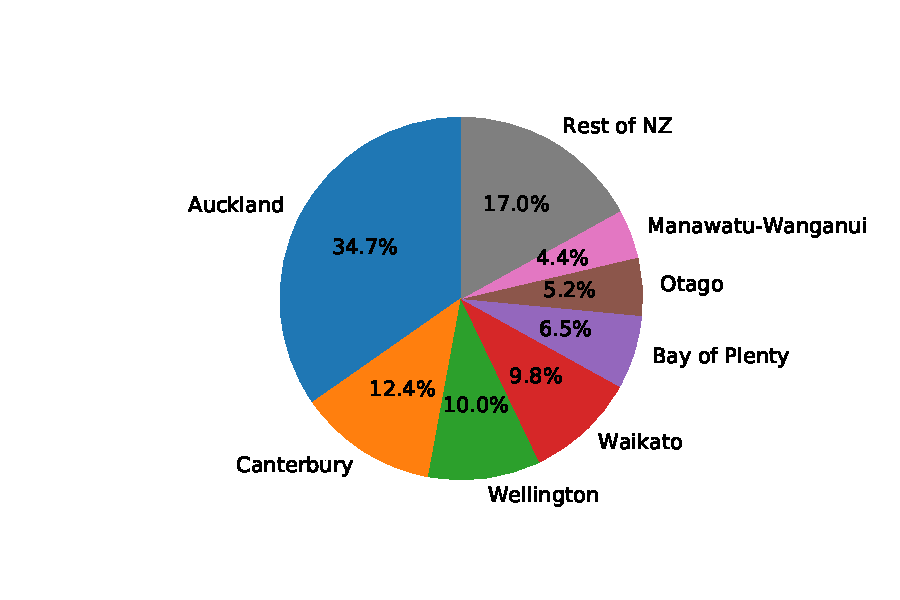
\includegraphics[width=1\linewidth]{PieTot_2020} \medskip \\
	\end{minipage}
}\hfill
\subfloat[Transport \& storage\label{fig:PieDistrib}]{
	\begin{minipage}[t]{0.30\linewidth}
	\centering
	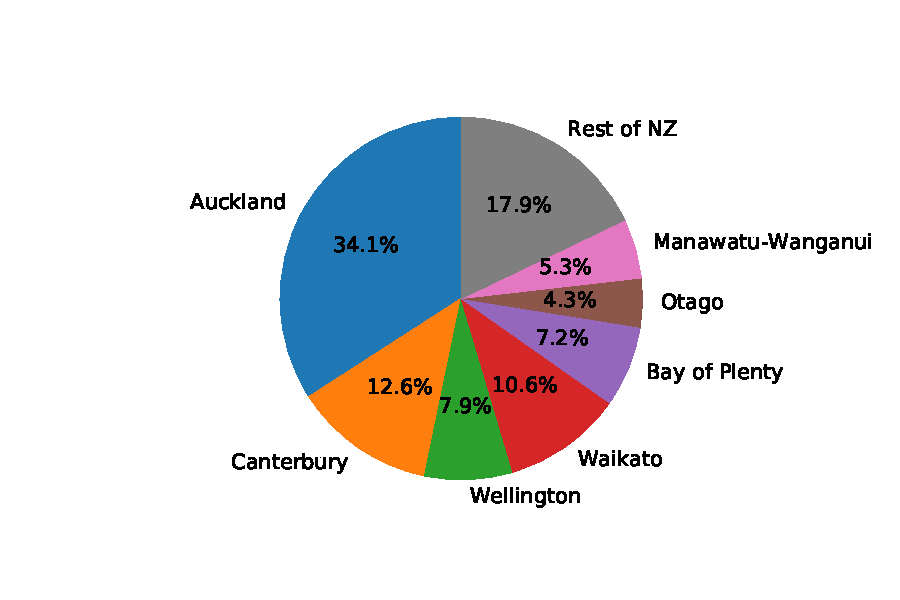
\includegraphics[width=1\linewidth]{PieDistr_2020} \medskip \\
	\end{minipage}
}\hfill
\subfloat[Wholesale \& retail\label{fig:PieSell}]{
	\begin{minipage}[t]{0.30\linewidth}
	\centering
	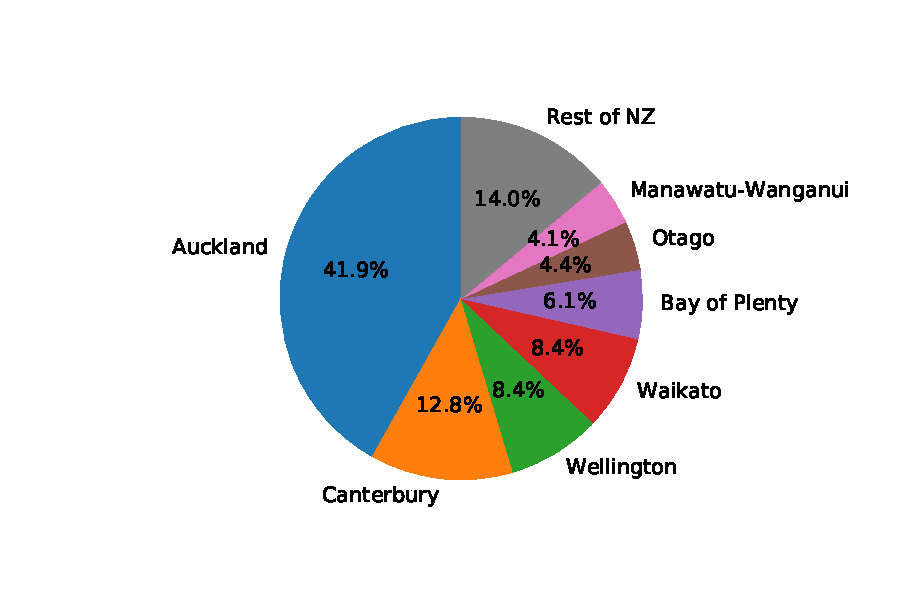
\includegraphics[width=1\linewidth]{PieSell_2020} \medskip \\
	\end{minipage}}
\caption{Percentage of national facilities in each region (2020)}\label{fig:PercOfFac}
\end{figure}
%

The contributions of the different regions have remained relatively stable in each area for each type of facility. 

\begin{table}[!h]
\caption{Some cap}\label{tab:regionCompLongit}
\resizebox{\textwidth}{!}{%
	\begin{tabular}{l c r r r r r c r r r r r c r r r r r c r c r}
	\toprule
	Region&&\multicolumn{5}{c}{All industries}&&\multicolumn{5}{c}{Distribution}&&\multicolumn{5}{c}{Selling}&&Pop&&GDP\\
	&&\rotatebox{90}{2000}&\rotatebox{90}{2005}&\rotatebox{90}{2010}&\rotatebox{90}{2015}&\rotatebox{90}{2020}&&\rotatebox{90}{2000}&\rotatebox{90}{2005}&\rotatebox{90}{2010}&\rotatebox{90}{2015}&\rotatebox{90}{2020}&&\rotatebox{90}{2000}&\rotatebox{90}{2005}&\rotatebox{90}{2010}&\rotatebox{90}{2015}&\rotatebox{90}{2020}&&2018&&2019\\
	\midrule
	Auckland&&30.3&31.4&31.4&33.2&34.7&&34.0&32.9&31.9&33.2&34.1&&37.3&38.4&39.0&41.6&41.9&&33.4&&37.6\\
	Canterbury&&12.3&12.5&12.6&12.9&12.4&&11.9&12.3&12.6&12.9&12.6&&13.3&13.5&13.5&12.9&12.8&&12.8&&12.4\\
	Waikato&&10.6&10.3&10.1&9.9&9.8&&10.1&10.5&10.5&10.1&10.6&&8.4&8.4&8.3&8.2&8.4&&9.7&&8.5\\
	Wellington&&10.5&10.1&10.2&10.0&10.0&&9.6&8.7&8.6&8.4&7.9&&10.4&9.6&9.3&8.8&8.4&&10.8&&12.9\\
	Bay of Plenty&&6.5&6.7&6.6&6.4&6.5&&7.0&6.9&7.0&6.8&7.2&&6.1&6.1&6.2&5.9&6.1&&6.6&&5.7\\
	Manawatu-Wanganui&&5.7&5.3&5.1&4.7&4.4&&6.0&6.1&5.9&5.5&5.3&&5.1&4.7&4.5&4.2&4.1&&5.1&&3.8\\
	Otago&&4.6&4.9&5.1&5.2&5.2&&4.1&4.6&4.6&4.4&4.3&&4.3&4.3&4.4&4.3&4.4&&4.8&&4.5\\
	Rest of NZ&&19.5&18.9&18.7&17.8&17.0&&17.3&18.0&18.9&18.6&17.9&&15.2&14.8&14.8&14.0&14.0&&16.8&&14.7\\
	\bottomrule
	\end{tabular}}

\end{table}



\nmt{Next look at growth rates and birth/death rates of facilities (first need to create C stats)}

\section{Regions in spatial detail}
Only Auckland, Canterbury, Wellington, Waikato

\section{The communities who pay}

\subsection{Data}

\section*{References}
\bibliography{logisticSprawl_NZ}


\end{document}
